\documentclass[12pt,a4paper]{article}
\usepackage[utf8]{inputenc}
\usepackage[T1]{fontenc}
\usepackage[margin=2.54cm]{geometry}
\usepackage{amssymb}
\usepackage{graphicx}
\usepackage{amsmath}
\usepackage{booktabs}
\usepackage{float}
\usepackage{ctex}
\usepackage{multirow}
\usepackage{pifont}
\usepackage{xcolor}
\usepackage{titlesec}
\titleformat{\section}[block]{\centering\large\bfseries}{\chinese{section}}{1em}{}
\titleformat{\subsection}{\normalfont\large\bfseries}{\arabic{section}.\arabic{subsection}}{1em}{}
\titleformat{\subsubsection}{\normalfont\normalsize\bfseries}{\arabic{section}.\arabic{subsection}.\arabic{subsubsection}}{1em}{}
\usepackage{listings}
\lstset{
	language=C,
	basicstyle=\ttfamily,
	keywordstyle=\color{blue}, 
	commentstyle=\color{green!40!black},
	stringstyle=\color{orange}, 
	numbers=left,
	numberstyle=\tiny\color{gray},
	breaklines=true,
	frame=single,
	tabsize=4
}
\begin{document}
		
		\title{\textbf{多波束测量的测线优化模型}\\[-2.5em]}
		\author{}
		\date{}
		\maketitle
		\thispagestyle{empty}
		\begin{quote}
			
			\begin{center}
				\textbf{\zihao{4}摘要}\medskip
			\end{center}
			
			\hspace{1.75em} 多波束测深系统是单波束测深的进一步发展,它具有更高的精度和测量效率。多波束测深系统在同一时间内可以发射多个声波束,然后接收从不同方向返回的声波信号。在真实海底地形中,地形起伏变化较大。因此,需要根据具体海域的地形情况,合理设计测线间距,以平衡重叠率和测量效率。这涉及到在不同水深区域采用不同的测量策略,以获得最佳的测量结果。
			
			\hspace{1.75em}\textbf{问题一}:海底坡面与水平面存在夹角问题。针对问题一,以中心测量船下方的海底坡面为原点建立直角坐标系,并根据多波束换能器的开角,得到两侧波束的方程,根据两侧的方程以及海底坡面的方程,得到目标测量船与相邻测量船的两侧波束与海底坡面的交点。通过C计算得出问题1的结果,其中各测量船与前一条测线的重叠率(\%)分别为37.93、33.43 、27.89、...、-1.12、-12.22。
			
			\hspace{1.75em}\textbf{问题二}:测线方向与海底坡面之间夹角可变问题。针对问题二,以中心测量船下方的海底坡面为原点建立三维直角坐标系,同样根据海底坡面的法向量和经过原点求得海底坡面的方程,并且目标测量船两侧波束的角度已知,联立方程通过C求解得到问题2的结果,在测线方向夹角为0°的时候,测量船随着每0.3海里的增加,覆盖宽度依次为415.69、466.09、516.49、566.89、...、768.48米。
			
			\hspace{1.75em}\textbf{问题三}:以测量长度最小为目标的测线设计问题。针对问题三,该问题为动态规划问题,将该问题转变为单位测线长度扫描的海域面积尽可能大和扫描的海域面积与上一次扫描的海域重叠部分尽可能小两个目标,并且约束条件有覆盖率在10\%$\sim$20\%之间。得出测线总长77912.95米,使用的测量船为18辆。
			
			\hspace{1.75em}\textbf{问题四}:多目标测线设计问题。针对问题四,在问题三的基础上引入覆盖率超过20\%长度尽可能短的目标,在问题三的基础上,去除覆盖率在10\%$\sim$20\%之间的约束,并且海水深度通过已知数据的三维拟合得出。最优测线的测线总长度为392497.43米,侧漏海区占总待测海域面积的漏测率8.46\%,重叠率超过20\%部分的总长度为5642.33米
			
			\hspace{1.75em}最后,对模型进行评价和推广,并对换能器开角参数进行灵敏度分析。
			\bigskip
			
			\textbf{关键词:多波束测量的测线优化;多目标优化;动态优化;直角坐标系}
		\end{quote}
	\clearpage
	\setcounter{page}{1}
	
	
	\section{问题重述}
\subsection{背景介绍}
	单波束测深和多波束测深是两种水下深度测量技术,它们利用声波在水中的传播原理来测定水体深度。声波在均匀介质中以匀速直线传播,并在不同界面上产生反射,这一基本原理为测深技术的核心。
	
	\noindent\textbf{多波束测深}
	
	多波束测深系统是单波束测深的进一步发展,它具有更高的精度和测量效率。多波束测深系统在同一时间内可以发射多个声波束,然后接收从不同方向返回的声波信号。其工作原理如下:多波束测深系统可以同时发射多个声波束,每个声波束具有不同的方向。接收器捕获从不同方向返回的声波信号。这使得系统可以获得更多关于水底地形的信息。通过处理多个声波束的返回信号,系统可以更准确地确定水体深度和地形特征。
	
	\noindent\textbf{重叠率的重要性}
	
	在多波束测深中,覆盖宽度$W$随着发射角度$\theta$和水深$D$的变化而变化。为了确保测量的准确性和数据的完整性,相邻条带之间应具有一定的重叠率$\eta$,通常为 10\%$\sim$20\%。这可以避免数据缺失或冗余,确保测量结果的可靠性。
	
	然而,在真实海底地形中,地形起伏变化较大。因此,需要根据具体海域的地形情况,合理设计测线间距,以平衡重叠率和测量效率。这涉及到在不同水深区域采用不同的测量策略,以获得最佳的测量结果。
	
	\subsection{问题介绍}
	问题 1:对于与测线方向垂直的平面和海底坡面的交线,形成一条斜线,其与水平面的夹角称为坡度$\alpha$。请建立多波束测深的覆盖宽度和相邻条带之间重叠率的数学模型。假设多波束换能器的开角为120度,坡度为1.5度,而海域中心点处的海水深度为70米。请使用模型计算表格中所列位置的参数值,并将结果格式化如表格所示,同时保存到result1.xlsx文件中。
	
	问题 2:考虑一个矩形待测海域,其中测线方向与海底坡面法线在水平面上的投影夹角为$\beta$。请建立多波束测深覆盖宽度的数学模型。假设多波束换能器的开角为120度,坡度为1.5度,而海域中心点处的海水深度为120米。使用模型计算表格中所列位置的多波束测深覆盖宽度,并将结果格式化如表格所示,保存到result2.xlsx文件中。
	
	问题 3:在一个南北长2海里、东西宽4海里的矩形海域内,中心点的海水深度为110米,呈现出西深东浅的坡度,多波束换能器的开角为120度。请设计一组最短的测线,以完全覆盖整个待测海域,同时满足相邻条带之间10\%$\sim$20\%的重叠率要求。
	
	问题 4:附件.xlsx中包含若干年前某海域的单波束测深数据。现在希望利用这组数据来协助设计多波束测量船的测量布局。设计测线时,请考虑以下要求:(1)沿测线形成的条带尽可能覆盖整个待测海域;(2)相邻条带之间的重叠率尽量不超过20\%;(3)测线总长度最短。设计测线后,请计算以下指标:(1)测线的总长度;(2)漏测海区占总待测海域面积的百分比;(3)在重叠区域内,重叠率超过20\%部分的总长度。
	
	\section{问题分析}
	\subsection{问题一分析}
	为了计算多波束测深的覆盖宽度以及和相邻条带之间的重叠率,并且由于海底坡面与水平面具有大小$\alpha$的夹角,并且多波束焕能器的开角是已知的,可以建立对应的直角坐标系进行求解,求解两个开角的波束方程和海底坡面的直线方程,得就能够求得每个交点的坐标,进而求得多波束测深的覆盖宽度和相邻条带之间重叠率。
	
	\subsection{问题二分析}
	问题一考虑的是测线方向与坡面的法向量在水平面上投影夹角为90°的情况,但是真实情况往往是不同的,因此需要在问题一的基础上转为建立三维的坐标系方程,同样求得那些交点的坐标,继而获得目标测量船的覆盖宽度。在三维的坐标系中,平面方程由一个点的坐标与法向量计算得到,直线方程由一个点的坐标与方向向量得到。
	\subsection{问题三分析}
	问题三考虑在一个固定海域中进行多波束策测量,目的是要使得整条测试线的长度尽可能短,对于该问题来说,其实本质上就是一个以总测量长度最短为目标的优化模型,存在的约束分贝有重叠率的约束、覆盖整个海域的约束等。对于该问题最好的求解方法还是进行三维直角坐标系的建立。
	\subsection{问题四分析}
	问题四在问题三的基础上进行改进,主要改变的地方有海底坡面不再是固定的角度或者曲线,而是有一些具体的测量的点,因此我们计算在海底坡面的投影与上问中存在区别,还有一个区别就是第三问中设计的条带只需要满足测量长度最短,在第四问中需要新增两个目标函数。
	
\section{模型假设}
	
	假设不同条带之间不一定是平行的;
	
	假设附件中给出的数据是真实可靠的;
	
	假设在多波束测深系统运行的过程中,不存在恶劣天气或设备故障对于测量结果的影响;
	
	假设在多波束测深系统运行的过程中,所有测量船都会根据预先计划好的方向进行行进,整个系统不受外界的干扰。
	
	\section{符号说明}
	
\begin{center}
		\begin{tabular}{cc}
	\toprule 符号 & 符号说明 \\
	\midrule$d_A$ & 目标测量船 A 与中心测量船之间的距离 \\
		$D_A$ & 目标测量船 A 所处的海水深度 \\
		$D$ & 中心测量船处的海水深度 \\
		$W_A$ & 目标测量船 $\mathrm{A}$ 的覆盖宽度 \\
		$\eta_A$ & 目标测量船 $\mathrm{A}$ 与相邻测量船 $\mathrm{B}$ 之间的重叠率 \\
		$n$ & 当前规划测线的次数 \\
		$S n$ & 第 $n$ 次规划测线扫描到的有效海域面积 \\
		$L n$ & 第 $n$ 次规划测线的总长 \\
		 $IOUn$ & 第 $n$ 次扫描的海域与第 $n-1$ 次扫描的海域重叠面积 \\
		$R S_{P s n}$ & 扫描船在从 $P s_n$ 向 $P t_n$ 扫描的过程中,右半侧扫描带宽 \\
		\bottomrule
	\end{tabular}
\end{center}
	
\section{问题一模型的建立与求解}
	\subsection{问题一分析}
	为了计算多波束测深的覆盖宽度以及和相邻条带之间的重叠率,并且由于海底坡面与水平面具有大小$\alpha$的夹角,并且多波束焕能器的开角是已知的,可以建立对应的直角坐标系进行求解,求解两个开角的波束方程和海底坡面的直线方程,得就能够求得每个交点的坐标,进而求得多波束测深的覆盖宽度和相邻条带之间重叠率。
\subsection{直角坐标系建立}
	下图为问题1中所有测量船分布以及海底面情况的示意图,在该图中,需要求解的目标变量为测量船A处的海水深度、测量船A的覆盖宽度和测量船A与测量船B的重叠率。
	\begin{figure}[H]
		\centering
		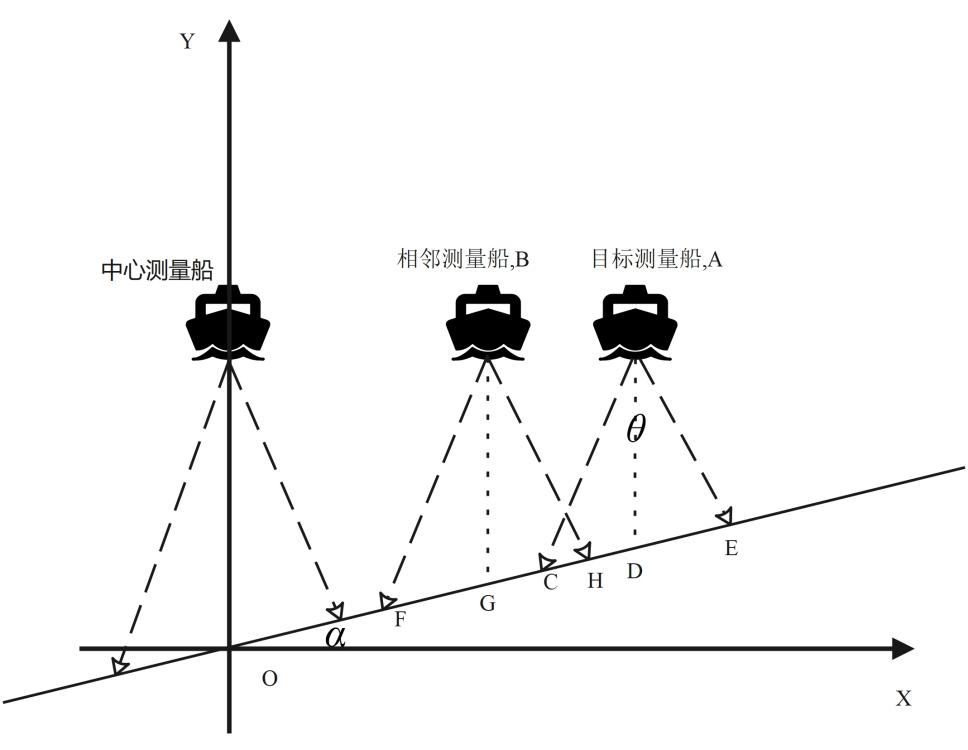
\includegraphics[width=0.8\linewidth]{media/image7}
		\caption{问题1的示意图}
		\label{fig1}
	\end{figure}
	
	\subsection{多波束测深指标建模}
	直线CD为海底面,其直线方程由与x轴正方向的夹角大小得出,海底面方程为:
	$$
	y_{\text {海底 }}=\tan (\alpha) x
	$$
	
	目标测量船 $\mathrm{A}$ 与中心测量船之间的距离是已知的, 假设为 $d_A$, 那么 $\mathrm{D}$ 点的 坐标为:
	$$
	\left(x_D, y_D\right)=\left(d_A, \tan (\alpha) d_A\right)
	$$
	那么, 目标测量船 $\mathrm{A}$ 所处的海水深度 $D_A$, 式中 $D$ 表示中心测量船处的海水 深度:
	$$
	D_A=D-\tan (\alpha) d_A
	$$
	
	对于目标测量船A来说,覆盖宽度就是线段CE的长度,其中,线段AC所在的直线满足方程:
	$$
	\left(y_{A C}-D\right)=\tan \left(\frac{3 \pi-\theta}{2}\right)\left(x-d_A\right)
	$$
	线段 $\mathrm{AE}$ 所在的直线满足方程:
	$$
	\left(y_{A E}-D\right)=\tan \left(\frac{3 \pi+\theta}{2}\right)\left(x-d_A\right)
	$$
	根据海底面方程以及直线 $\mathrm{AC}$ 的方程求得 $\mathrm{C}$ 点的坐标 $\left(x_C, y_C\right)$, 根据海底面 方程以及直线 $\mathrm{AE}$ 的方程求得 $\mathrm{E}$ 点的坐标 $\left(x_E, y_E\right)$, 此时目标测量船 $\mathrm{A}$ 的覆盖宽 度 $W_A$ 就为 $\mathrm{CE}$ 的长度为:
	$$
	W_A=\sqrt{\left(x_C-x_E\right)^2+\left(y_C-y_E\right)^2}
	$$
	
	目标测量船A与相邻测量船B条带之间的重叠率定义为向量CH与向量CE的比值,具体来说,就是(HF+CE-FE)/CE,因此需要获得BF和BH的方程,线段BF所在直线满足方程,式中$d$表示相邻两个测量船之间的距离:
	$$
	\left(y_{A C}-(D-d)\right)=\tan \left(\frac{3 \pi-\theta}{2}\right)\left(x-d_A\right)
	$$
	
	线段 BH 所在的直线满足方程:
	$$
	\left(y_{A E}-(D-d)\right)=\tan \left(\frac{3 \pi+\theta}{2}\right)\left(x-d_A\right)
	$$
	
	根据海底面方程以及直线BF的方程求得F点的坐标$\left( {{x}_{F}},{{y}_{F}} \right)$,根据海底面方程以及直线BH的方程求得H点的坐标$\left( {{x}_{H}},{{y}_{H}} \right)$,因此目标测量船A与测量船B之间的重叠率${{\eta }_{A}}$为:
	$$
	\eta_A=\frac{\sqrt{\left(x_F-x_H\right)^2+\left(y_F-y_H\right)^2}+\sqrt{\left(x_C-x_E\right)^2+\left(y_C-y_E\right)^2}-\sqrt{\left(x_F-x_E\right)^2+\left(y_F-y_E\right)^2}}{W_A}
	$$
	
	\subsection{多波束测深指标求解}
	考虑一个多波束测深系统,在该系统中,多波束换能器的开角为120°,坡度的大小为1.5°,测量船之间距离均为200米,并且中心处的海水深度为70m,计算此时每个测量船的海水深度、覆盖宽度和与前一条测线的重叠率这些评价多波束测深的指标。
	
	根据给定的参数条件以及上文中的建模过程,得到问题1的计算结果如下表所示,其中各测量船与前一条测线的重叠率(\%)分别为37.93、33.43 、27.89、...、-1.12、-12.22,随着海水深度变浅,与前一条测线的重叠率也在不断变小。
	\begin{table}[H]
		\centering
		\caption{问题1的结果}
		\label{tab1}
		\begin{tabular}{@{}cccc@{}}
			\toprule
			\begin{tabular}[c]{@{}c@{}}测线距中心点处\\ 的距离/m\end{tabular} & 海水深度/m & 覆盖宽度/m & \begin{tabular}[c]{@{}c@{}}与前一条测线的重\\ 叠率/\%\end{tabular} \\ \midrule
			-800 & 90.95 & 315.81 & --     \\
			-600 & 85.71 & 297.63 & 37.93  \\
			-400 & 80.47 & 279.44 & 33.43  \\
			-200 & 75.24 & 261.26 & 27.89  \\
			0    & 70.00 & 243.07 & 22.50  \\
			200  & 64.76 & 224.88 & 14.85  \\
			400  & 59.53 & 206.70 & 7.92   \\
			600  & 54.29 & 188.51 & -1.12  \\
			800  & 49.05 & 170.33 & -12.22 \\ \bottomrule
		\end{tabular}
	\end{table}
	
\section{问题二模型的建立与求解}
	\subsection{问题二分析}
	问题一考虑的是测线方向与坡面的法向量在水平面上投影夹角为90°的情况,但是真实情况往往是不同的,因此需要在问题一的基础上转为建立三维的坐标系方程,同样求得那些交点的坐标,继而获得目标测量船的覆盖宽度。在三维的坐标系中,平面方程由一个点的坐标与法向量计算得到,直线方程由一个点的坐标与方向向量得到。
	\subsection{三维直角坐标系建立}
	问题2考虑了航线方向(测线方向)是可变的情况,这样就使得整个多波束测深的系统增加了侧方向的维度,即系统的维度从二维变成了三维,同样地,以中心测量船下方的海底点为原点,建立三维的直角坐标系,下图为问题2的示意图。
	\begin{figure}[H]
		\centering
		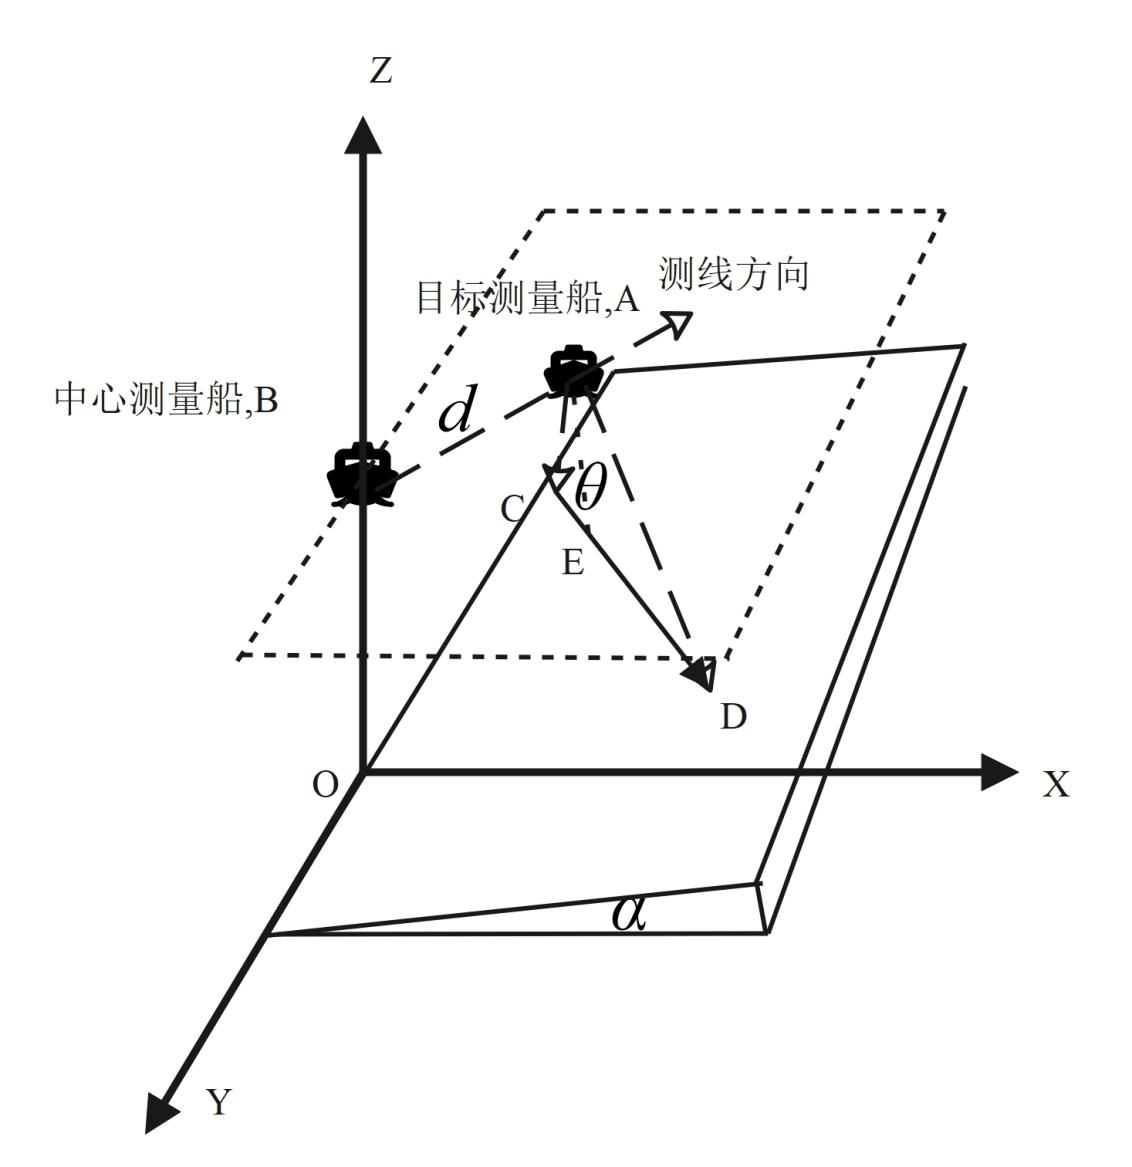
\includegraphics[width=0.8\linewidth]{media/image22}
		\caption{问题二的示意图}
		\label{fig2}
	\end{figure}

上图为问题二的示意图以及建立的对应的三维直角坐标系,其中需要求的覆盖宽度就是图中线段CD的长度,目标测量船A可以看做是从中心测量船B开行一段时间后的位置,AB之间的长度定义为${{d}_{A}}$。

\subsection{多波束测深覆盖宽度建模}
为了计算目标测量船A的覆盖宽度,其基本原理就是求线段CD的长度,即需要求得C和D的坐标,其中点C的坐标可以看做是直线AC与平面OCD的交点,而点D可以看做是直线AD与平面OCD的交点。

对于海底坡面平面OCD来说,其经过原点(0,0,0),并且由于平面与XOY平面的夹角为 $\alpha$, 因此该平面的法向量为 $(0, \tan (\alpha), 1)$, 因此海底坡面OCD的方程为:
$$
\tan (\alpha) y_{\text {海底 }}+z_{\text {海底 }}=0
$$

根据直线AC的方程以及海底坡面OCD的方程,得出C点的坐标$\left( {{x}_{C}},{{y}_{C}},{{z}_{C}} \right)$。

对于AC所在的直线来说,首先其经过点A$\left( {{d}_{A}}\sin \left( \beta  \right),{{d}_{A}}\cos \left( \beta  \right),D \right)$,其次,假设一个从A开始,沿着AC方向的单位向量,求该单位向量就是求直线AC的方向向量。首先AE是始终竖直向下的,因此该单位向量总能够在Z轴上得到分量$-\cos \left( \frac{\theta }{2} \right)$,在XOY平面上的分量为$\sin \left( \frac{\theta }{2} \right)$,根据测线方向与海底坡面的法向量在水平面上投影的夹角为$\beta $,因此ABY的角度为$\beta $,在XOY平面中,YAC的角度为$\beta +\frac{\pi }{2}$,因此该单位向量的向量取值为$\left( \sin \left( \frac{\theta }{2} \right)\cos \left( \beta  \right),-\sin \left( \frac{\theta }{2} \right)\sin \left( \beta  \right),-\cos \left( \frac{\theta }{2} \right) \right)$。因此直线AC的所在的方程为:
$$
\frac{x_{A C}-d_A \sin (\beta)}{\sin \left(\frac{\theta}{2}\right) \cos (\beta)}=\frac{y_{A C}-d_A \cos (\beta)}{-\sin \left(\frac{\theta}{2}\right) \sin (\beta)}=\frac{z_{A C}-D}{-\cos \left(\frac{\theta}{2}\right)}
$$

根据直线AC的方程以及海底坡面OCD的方程,得出C点的坐标$\left( {{x}_{C}},{{y}_{C}},{{z}_{C}} \right)$。

对于AD所在的直线来说,首先其经过点A$\left( {{d}_{A}}\sin \left( \beta  \right),{{d}_{A}}\cos \left( \beta  \right),D \right)$,其次,假设一个从A开始,沿着AD方向的单位向量,求该单位向量就是求直线AD的方向向量。首先AE是始终竖直向下的,因此该单位向量总能够在Z轴上得到分量$-\cos \left( \frac{\theta }{2} \right)$,在XOY平面上的分量为$\sin \left( \frac{\theta }{2} \right)$,根据测线方向与海底坡面的法向量在水平面上投影的夹角为$\beta $,因此ABY的角度为$\beta $,在XOY平面中,YAD的角度为$\beta -\frac{\pi }{2}$,因此该单位向量的向量取值为$\left( -\sin \left( \frac{\theta }{2} \right)\cos \left( \beta  \right),\sin \left( \frac{\theta }{2} \right)\sin \left( \beta  \right),-\cos \left( \frac{\theta }{2} \right) \right)$。因此直线AD的所在的方程为:
$$
\frac{x_{A C}-d_A \sin (\beta)}{-\sin \left(\frac{\theta}{2}\right) \cos (\beta)}=\frac{y_{A C}-d_A \cos (\beta)}{\sin \left(\frac{\theta}{2}\right) \sin (\beta)}=\frac{z_{A C}-D}{-\cos \left(\frac{\theta}{2}\right)}
$$

根据直线AD的方程以及海底坡面OCD的方程,得出D点的坐标$\left( {{x}_{D}},{{y}_{D}},{{z}_{D}} \right)$。

计算出C点坐标以及D点坐标之后,目标测量船A的覆盖宽度${{W}_{A}}$就为:
$$
W_A=\sqrt{\left(x_D-x_C\right)^2+\left(y_D-y_C\right)^2+\left(z_D-z_C\right)^2}
$$

\subsection{多波束测深覆盖宽度模型的求解}
考虑一个多波束测深系统,在该系统中,多波束换能器的开角为120°,坡度的大小为1.5°,中心处的海水深度为120m,计算此时每个测量船的覆盖宽度如何随着距离海域中心为距离以及测线方向夹角的变化而变化的。

根据给定的参数条件以及上文中的建模过程,得到问题2的计算结果如下表所示,其中,在测线方向夹角为0°的时候,测量船随着每0.3海里的增加,覆盖宽度依次为415.69、466.09、516.49、566.89、...、768.48米。
\begin{table}[H]
	\centering
	\caption{问题2的结果}
	\label{tab2}
	\begin{tabular}{|cc|cccccccc|}
		\hline
		\multicolumn{2}{|c|}{\multirow{2}{*}{\begin{tabular}[c]{@{}c@{}}覆盖\\ 宽度/m\end{tabular}}} &
		\multicolumn{8}{c|}{测量船距海域中心点处的距离/海里} \\ \cline{3-10} 
		\multicolumn{2}{|c|}{} &
		\multicolumn{1}{c|}{0} &
		\multicolumn{1}{c|}{0.3} &
		\multicolumn{1}{c|}{0.6} &
		\multicolumn{1}{c|}{0.9} &
		\multicolumn{1}{c|}{1.2} &
		\multicolumn{1}{c|}{1.5} &
		\multicolumn{1}{c|}{1.8} &
		2.1 \\ \hline
		\multicolumn{1}{|c|}{\multirow{8}{*}{\begin{tabular}[c]{@{}c@{}}测\\ 线\\ 方\\ 向\\ 夹\\ 角\\ /°\end{tabular}}} &
		0 &
		\multicolumn{1}{c|}{415.69} &
		\multicolumn{1}{c|}{466.09} &
		\multicolumn{1}{c|}{516.49} &
		\multicolumn{1}{c|}{566.89} &
		\multicolumn{1}{c|}{617.29} &
		\multicolumn{1}{c|}{667.69} &
		\multicolumn{1}{c|}{718.09} &
		768.48 \\ \cline{2-10} 
		\multicolumn{1}{|c|}{} &
		45 &
		\multicolumn{1}{c|}{422.85} &
		\multicolumn{1}{c|}{459.10} &
		\multicolumn{1}{c|}{495.35} &
		\multicolumn{1}{c|}{531.60} &
		\multicolumn{1}{c|}{567.85} &
		\multicolumn{1}{c|}{604.10} &
		\multicolumn{1}{c|}{640.35} &
		676.60 \\ \cline{2-10} 
		\multicolumn{1}{|c|}{} &
		90 &
		\multicolumn{1}{c|}{416.55} &
		\multicolumn{1}{c|}{416.55} &
		\multicolumn{1}{c|}{416.55} &
		\multicolumn{1}{c|}{416.55} &
		\multicolumn{1}{c|}{416.55} &
		\multicolumn{1}{c|}{416.55} &
		\multicolumn{1}{c|}{416.55} &
		416.55 \\ \cline{2-10} 
		\multicolumn{1}{|c|}{} &
		135 &
		\multicolumn{1}{c|}{422.85} &
		\multicolumn{1}{c|}{386.59} &
		\multicolumn{1}{c|}{350.34} &
		\multicolumn{1}{c|}{314.09} &
		\multicolumn{1}{c|}{277.84} &
		\multicolumn{1}{c|}{241.59} &
		\multicolumn{1}{c|}{205.34} &
		169.09 \\ \cline{2-10} 
		\multicolumn{1}{|c|}{} &
		180 &
		\multicolumn{1}{c|}{415.69} &
		\multicolumn{1}{c|}{365.29} &
		\multicolumn{1}{c|}{314.89} &
		\multicolumn{1}{c|}{264.50} &
		\multicolumn{1}{c|}{214.10} &
		\multicolumn{1}{c|}{163.70} &
		\multicolumn{1}{c|}{113.30} &
		62.90 \\ \cline{2-10} 
		\multicolumn{1}{|c|}{} &
		225 &
		\multicolumn{1}{c|}{409.50} &
		\multicolumn{1}{c|}{374.40} &
		\multicolumn{1}{c|}{339.29} &
		\multicolumn{1}{c|}{304.18} &
		\multicolumn{1}{c|}{269.08} &
		\multicolumn{1}{c|}{233.97} &
		\multicolumn{1}{c|}{198.86} &
		163.76 \\ \cline{2-10} 
		\multicolumn{1}{|c|}{} &
		270 &
		\multicolumn{1}{c|}{416.55} &
		\multicolumn{1}{c|}{416.55} &
		\multicolumn{1}{c|}{416.55} &
		\multicolumn{1}{c|}{416.55} &
		\multicolumn{1}{c|}{416.55} &
		\multicolumn{1}{c|}{416.55} &
		\multicolumn{1}{c|}{416.55} &
		416.55 \\ \cline{2-10} 
		\multicolumn{1}{|c|}{} &
		315 &
		\multicolumn{1}{c|}{409.50} &
		\multicolumn{1}{c|}{444.61} &
		\multicolumn{1}{c|}{479.72} &
		\multicolumn{1}{c|}{514.82} &
		\multicolumn{1}{c|}{549.93} &
		\multicolumn{1}{c|}{585.04} &
		\multicolumn{1}{c|}{620.14} &
		655.25 \\ \hline
	\end{tabular}
\end{table}


\section{问题三模型的建立与求解}
\subsection{问题三分析}
问题三考虑在一个固定海域中进行多波束策测量,目的是要使得整条测试线的长度尽可能短,对于该问题来说,其实本质上就是一个以总测量长度最短为目标的优化模型,存在的约束分贝有重叠率的约束、覆盖整个海域的约束等。对于该问题最好的求解方法还是进行三维直角坐标系的建立。
\subsection{三维坐标系的建立}
为了方便建模以及变量的计算等过程,对问题三所研究的水域建立三维直角坐标系,下图为问题3的示意图。
\begin{figure}[H]
	\centering
	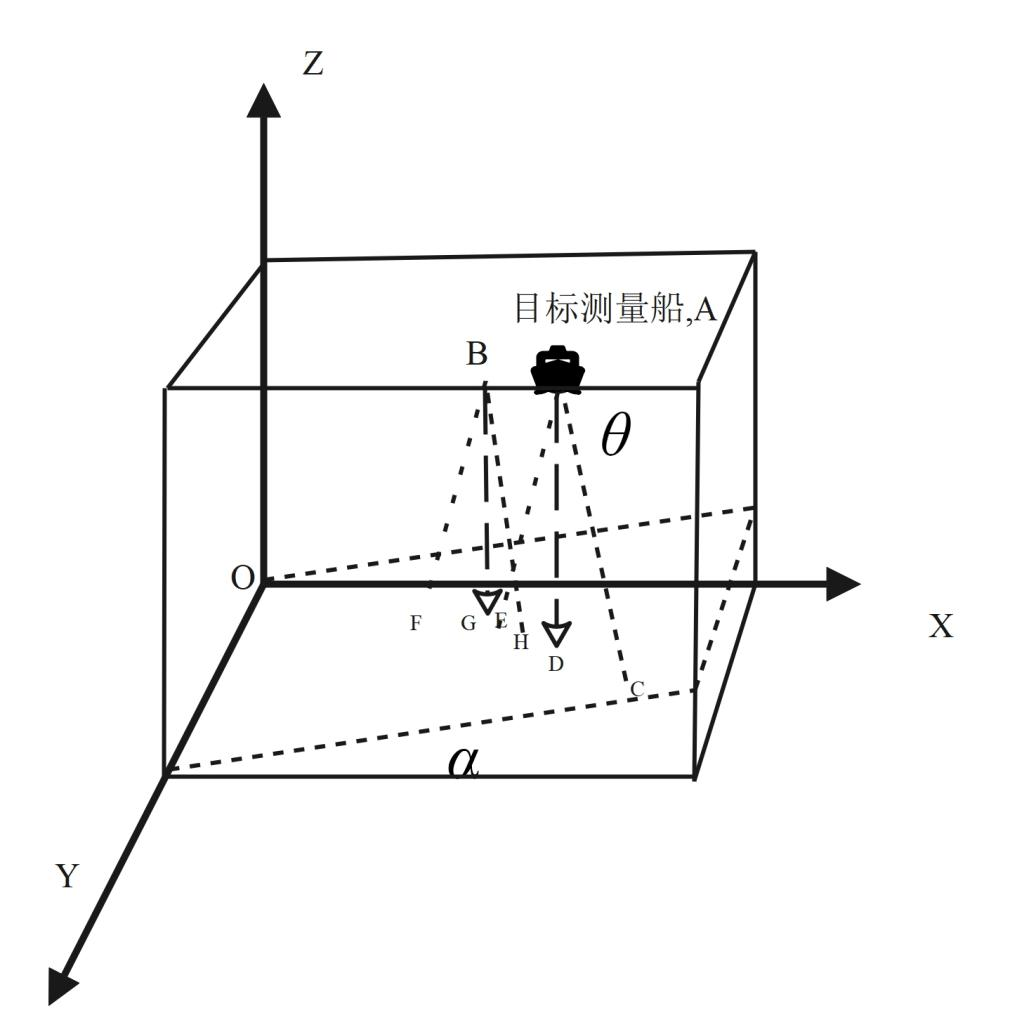
\includegraphics[width=0.8\linewidth]{media/image41}
	\caption{问题三的示意图}
	\label{fig3}
\end{figure}

在上图中,XOY表示水平面,OCE表示海底坡面所在的平面,其中A表示目标测量船,B表示与A 相邻的测量船,B在海底坡面上的波束点为F和H,A在海底坡面上的波束对面为E和C,并且EGFHDC六个点均在一个平面上。

\subsection{优化模型的建立}
为了尽可能提高海域扫描的效率,通过动态规划建立模型,每求解一次模型规划一条测线,直至完成对整个海域的扫描。

由于动态规划一定程度上会欠缺全局性,这里我们设置两个优化目标,进行多目标优化,以确保每一条规划的测线都尽可能达到最优。

目标函数1:希望单位测线长度扫描的海域面积尽可能大
$$
\max f_{n, 1}=\max \left\{\frac{S_n}{L_n}\right\}
$$

	式中$n$表示当前规划测线的次数。
	
	Sn表示第n次规划测线扫描到的\textbf{有效}海域面积(不包含超出海域范围的部分)。
	
	Ln表示第n次规划测线的总长(包含超出海域范围的部分)。
	
	目标函数2:希望扫描的海域面积与上一次扫描的海域重叠部分尽可能小。
	$$
	\max f_{n, 2}=\min \left\{I O U_n\right\}
	$$
	
	式中IOUn表示第n次扫描的海域与第n-1次扫描的海域重叠面积。最初一次扫描的重叠面积为0。
	
	\textbf{\ding{172}初次规划的约束条件:}
	\begin{figure}[H]
		\centering
		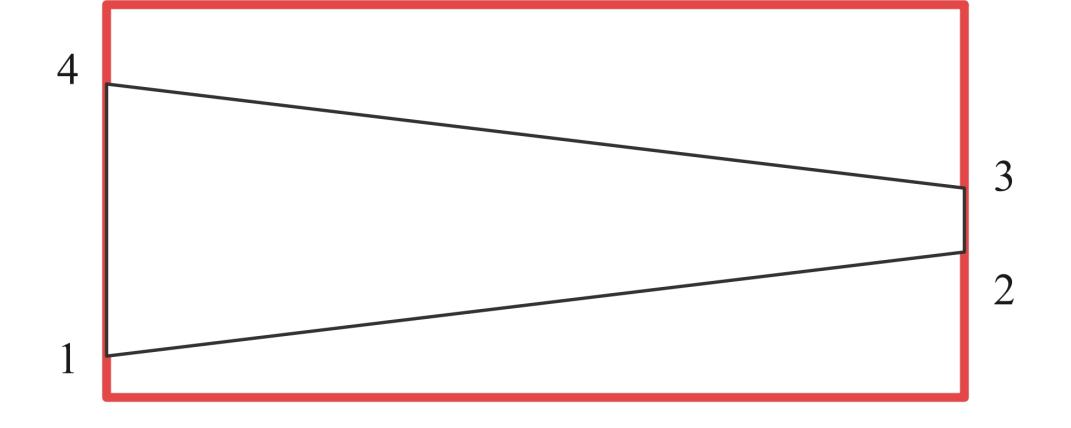
\includegraphics[width=0.75\linewidth]{media/image44}
		\caption{海底坡面示意图}
		\label{fig4}
	\end{figure}
	
	约束条件1:
	
	我们规定第一次规划测线,扫描的海域必须从包含矩形区域左下角顶点开始,结束时必须包含矩形区域的右下角顶点,以确定动态规划的初始条件。
	
	设扫描的海域四个顶点分别为 $\left(\mathrm{x}_{\mathrm{n}, 1}, \mathrm{y}_{\mathrm{n}, 1}\right) ;\left(\mathrm{x}_{\mathrm{n}, 2}, \mathrm{y}_{\mathrm{n}, 2}\right) ;\left(\mathrm{x}_{\mathrm{n}, 3}, \mathrm{y}_{\mathrm{n}, 3}\right) ;\left(\mathrm{x}_{\mathrm{n}, 4}, \mathrm{y}_{\mathrm{n}, 4}\right)$, 矩形区 域左下角顶点为 $\left(\mathrm{x}_{\mathrm{ld}}, \mathrm{y}_{\mathrm{ld}}\right)$, 右下角顶点为 $\left(\mathrm{x}_{\mathrm{rd}}, \mathrm{y}_{\mathrm{rd}}\right)$, 左上角顶点为 $\left(\mathrm{x}_{\mathrm{lu}}, \mathrm{y}_{\mathrm{lu}}\right)$, 右上角顶 点为 $\left(\mathrm{x}_{\mathrm{ru}}, \mathrm{y}_{\mathrm{ru}}\right)$
	$$
	\begin{aligned}
		& x_{1,1} \leq x_{l d}, y_{1,1} \leq y_{l d} \\
		& x_{1,2} \leq x_{r d}, y_{1,2} \leq y_{r d}
	\end{aligned}
	$$
	
	\textbf{\ding{173}第二次及之后规划的约束条件:}
	
	约束条件2:
	
	我们规定从第二次规划测线开始,每次扫描海域的四个顶点位置必须保证与前一次有交叠,并且需要保证交叠侧顶点不会发生漏测。
	$$
	\begin{gathered}
		x_{n, 1} \leq x_{n-1,4}, y_{n, 1} \leq y_{n-1,4}, n \geq 2 \\
		x_{n, 2} \leq x_{n-1,3}, y_{n, 2} \leq y_{n-1,3}, n \geq 2 \\
		x_{n, 1} \leq x_{l d}, n \geq 2 \\
		x_{n, 2} \geq x_{r d}, n \geq 2
	\end{gathered}
	$$
	
	约束条件3:
	
	重叠率不得超过20\%,也不得低于10\%。
	$$
	10 \% \leq \frac{I O U_n}{S_n} \leq 20 \%, n \geq 2
	$$
	
	\textbf{\ding{174}模型通用约束部分:}
	
	$
	\text { 决策变量为开始扫描的起点坐标 } P s_n\left(x_{n, P s}, y_{n, p s}\right) \text { 和终点坐标 } P t_n\left(x_{n, P t}, y_{n, p t}\right) 
	$,该坐标与梯形条带的四个顶点存在位置关系。
	
	约束条件4:
	
	梯形条带四个顶点与起点终点坐标之间的距离为定值。
	$$
	\begin{aligned}
		& \sqrt{\left(x_{n, 1}-x_{n, P s}\right)^2+\left(y_{n, 1}-y_{n, P s}\right)^2}=R S_{P_{S n}} \\
		& \sqrt{\left(x_{n, 1}-x_{n, P s}\right)^2+\left(y_{n, 1}-y_{n, P s}\right)^2}=R S_{P_{S n}} \\
		& \sqrt{\left(x_{n, 4}-x_{n, P s}\right)^2+\left(y_{n, 4}-y_{n, P s}\right)^2}=L S_{P_{S n}} \\
		& \sqrt{\left(x_{n, 2}-x_{n, P t}\right)^2+\left(y_{n, 2}-y_{n, P t}\right)^2}=R S_{P_{t n}} \\
		& \sqrt{\left(x_{n, 3}-x_{n, P t}\right)^2+\left(y_{n, 3}-y_{n, P t}\right)^2}=L S_{P_{t n}}
	\end{aligned}
	$$
	
	
	式中,$R S_{P s n}$、$R S_{P t n}$表示扫描船在从$\mathrm{Ps}_{\mathrm{n}}$ 向 $\mathrm{Pt}_{\mathrm{n}}$扫描的过程中,右半侧扫描带宽。左半侧扫描带宽则用数学符号的首字母为$L$。这四个值可以通过问题二的模型计算得到。
	
	约束条件5:
	
	扫描船的行驶方向垂直于扫描面。
	$$
	\begin{aligned}
		& \left(x_{n, 1}-x_{n, 4}\right)\left(x_{n, P s}-x_{n, P t}\right)+\left(y_{n, 1}-y_{n, 4}\right)\left(y_{n, P s}-y_{n, P t}\right)=0 \\
		& \left(x_{n, 2}-x_{n, 3}\right)\left(x_{n, P s}-x_{n, P t}\right)+\left(y_{n, 2}-y_{n, 3}\right)\left(y_{n, P s}-y_{n, P t}\right)=0
	\end{aligned}
	$$
	
	\textbf{\ding{175}动态规划模型的结束条件:}
	
	当下述条件被满足时,不再进行新一轮的规划。
	
	$$
	\begin{aligned}
		&\text{存在任意}n, \text{使得}\\
		& {\left[\left(x_{n, 1}-x_{n 1,4}\right)\left(y_{l u}-y_{n, 4}\right)-\left(x_{l u}-x_{n, 4}\right)\left(y_{n, 1}-y_{n, 4}\right)\right] \times} \\
		& {\left[\left(x_{n, 2}-x_{n 1,3}\right)\left(y_{l u}-y_{n, 3}\right)-\left(x_{l u}-x_{n, 3}\right)\left(y_{n, 2}-y_{n, 3}\right)\right] \geq 0 \text { 且 }} \\
		& {\left[\left(x_{n, 1}-x_{n 1,2}\right)\left(y_{l u}-y_{n, 2}\right)-\left(x_{l u}-x_{n, 2}\right)\left(y_{n, 1}-y_{n, 2}\right)\right] \times} \\
		& {\left[\left(x_{n, 3}-x_{n 1,4}\right)\left(y_{l u}-y_{n, 4}\right)-\left(x_{l u}-x_{n, 4}\right)\left(y_{n, 3}-y_{n, 4}\right)\right] \geq 0}
	\end{aligned}
	$$
	$$
	\begin{aligned}
		&\text{同时存在任意}m, \text{使得}\\
		& {\left[\left(x_{m, 1}-x_{m, 4}\right)\left(y_{r u}-y_{m, 4}\right)-\left(x_{r u}-x_{m, 4}\right)\left(y_{m, 1}-y_{m, 4}\right)\right] \times} \\
		& {\left[\left(x_{m, 2}-x_{m, 3}\right)\left(y_{r u}-y_{m, 3}\right)-\left(x_{r u}-x_{m, 3}\right)\left(y_{m, 2}-y_{m, 3}\right)\right] \geq 0 \text { 且 }} \\
		& {\left[\left(x_{m, 1}-x_{m, 2}\right)\left(y_{r u}-y_{m, 2}\right)-\left(x_{r u}-x_{m, 2}\right)\left(y_{m, 1}-y_{m, 2}\right)\right] \times} \\
		& {\left[\left(x_{m, 3}-x_{m, 4}\right)\left(y_{r u}-y_{m, 4}\right)-\left(x_{r u}-x_{m, 4}\right)\left(y_{m, 3}-y_{m, 4}\right)\right] \geq 0}
	\end{aligned}
	$$
	
	上述两个表达式表示矩形海域的另外两个顶点被包含在扫描海域中。
	
	综上所述,有希望单位测线长度扫描的海域面积尽可能大和扫描的海域面积与上一次扫描的海域重叠部分尽可能小的多目标动态规划模型:
	$$
	\begin{gathered}
		\max f_{n, 1}=\max \left\{\frac{S_n}{\left.L_n\right\}}\right. \\
		\max f_{n, 2}=\min \left\{I O U_n\right\} \\
		\text { s.t. }\left\{\begin{array}{l}
			x_{1,1} \leq x_{l d}, y_{1,1} \leq y_{l d} \\
			x_{1,2} \leq x_{r d}, y_{1,2} \leq y_{r d} \\
			x_{n, 1} \leq x_{n-1,4}, y_{n, 1} \leq y_{n-1,4}, n \geq 2 \\
			x_{n, 2} \leq x_{n-1,3}, y_{n, 2} \leq y_{n-1,3}, n \geq 2 \\
			x_{n, 1} \leq x_{l d}, n \geq 2 \\
			x_{n, 2} \geq x_{r d}, n \geq 2 \\
			10 \% \leq \frac{I O U_n}{S_n} \leq 20 \%, n \geq 2 \\
			\left(x_{n, 1}-x_{n, 4}\right)\left(x_{n, P s}-x_{n, P t}\right)+\left(y_{n, 1}-y_{n, 4}\right)\left(y_{n, P s}-y_{n, P t}\right)=0 \\
			\left(x_{n, 2}-x_{n, 3}\right)\left(x_{n, P_s}-x_{n, P t}\right)+\left(y_{n, 2}-y_{n, 3}\right)\left(y_{n, P s}-y_{n, P t}\right)=0
		\end{array}\right.
	\end{gathered}
	$$
	
	
	\subsection{优化模型的求解}
	针对上述多目标动态规划模型,采用C进行求解,得到多波束测深的示意图如下所示:
	\begin{figure}[H]
		\centering
		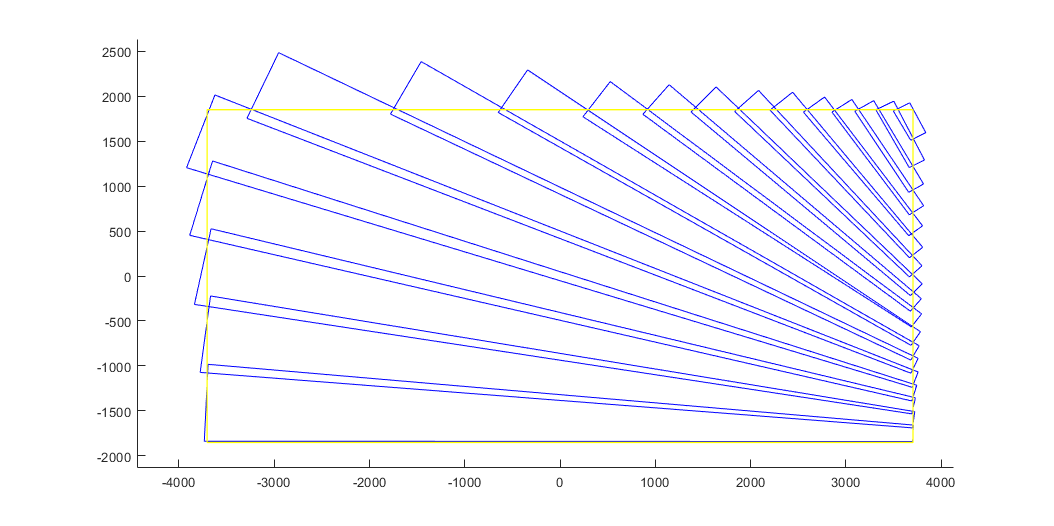
\includegraphics[width=0.5\linewidth]{media/image58}
		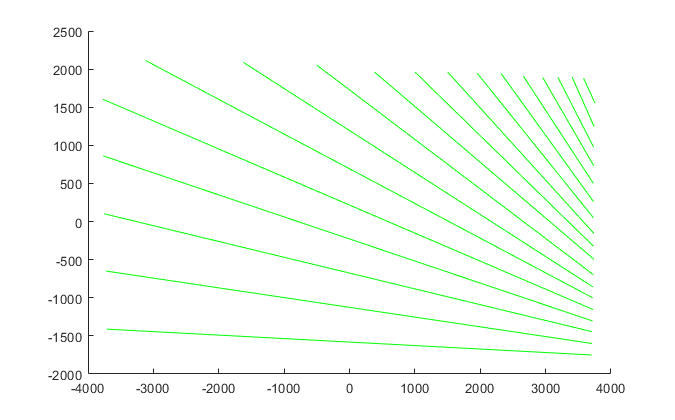
\includegraphics[width=0.4\linewidth]{media/image59}
		\caption{问题3的结果}
		\label{fig5}
	\end{figure}
	
	上面左图为多波束测深的条带示意图,上图右为测量长度的示意图,在这样最优的多波束测深系统中,测线总长77912.95米,使用的测量船为18辆。
	
	\section{问题四模型的建立与求解}
	\subsection{问题四分析}
	问题四在问题三的基础上进行改进,主要改变的地方有海底坡面不再是固定的角度或者曲线,而是有一些具体的测量的点,因此我们计算在海底坡面的投影与上问中存在区别,还有一个区别就是第三问中设计的条带只需要满足测量长度最短,在第四问中需要新增两个目标函数。
	\subsection{海底坡面的插值}
	由于海底坡面的方程不再知道,因此为了知道对应xy值的情况下,海水深度,需要通过已知采样点的值来对中间的海水深度进行插值,即采用相邻已知海水深度的坐标求得待测点的海水深度。
	\subsection{多目标动态规划模型的建立}
	目标函数1:希望单位测线长度扫描的海域面积尽可能大
	$$
	\max f_{n, 1}=\max \left\{\frac{S_n}{L_n}\right\}
	$$
	
	式中$n$表示当前规划测线的次数。
	
	Sn表示第n次规划测线扫描到的\textbf{有效}海域面积(不包含超出海域范围的部分)。
	
	Ln表示第n次规划测线的总长(包含超出海域范围的部分)。
	
	目标函数2:希望扫描的海域面积与上一次扫描的海域重叠部分尽可能小。
	$$
	\max f_{n, 2}=\min \left\{I O U_n\right\}
	$$
	
	式中IOUn表示第n次扫描的海域与第n-1次扫描的海域重叠面积。最初一次扫描的重叠面积为0。
	
	目标函数3:相邻条带之间的重叠率尽量不超过20\%
	$$
	\max f_{n, 3}=\min \left\{\frac{I O U_n}{S_n}-20 \%\right\} n \geq 2
	$$
	
	对于该多目标动态优化模型来说,其余第三问的约束条件主要区别在于海底坡面中距离的计算上以及缺少了问题三中,对于相邻条带之间的重叠率在10\%$\sim$20\%之间的约束。
	\subsection{多目标动态规划模型的求解}
	通过C进行求解,得到问题4中多波束测量的设计,具体的多波束测量系统的分布如下图所示。
	\begin{figure}[H]
		\centering
		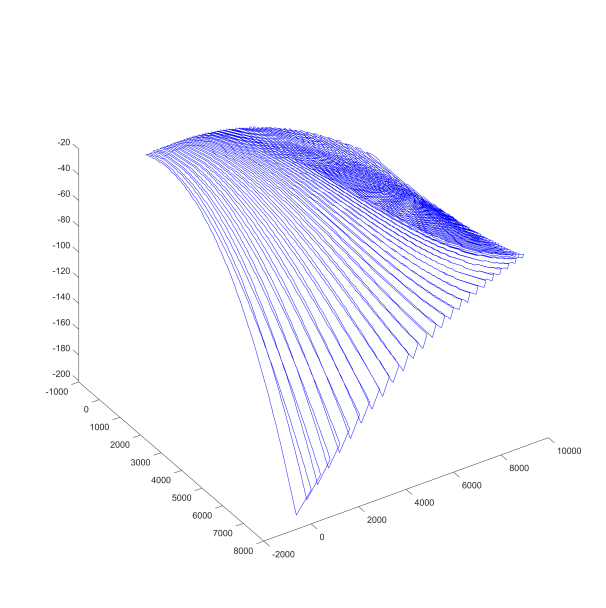
\includegraphics[width=0.5\linewidth]{media/image61}
		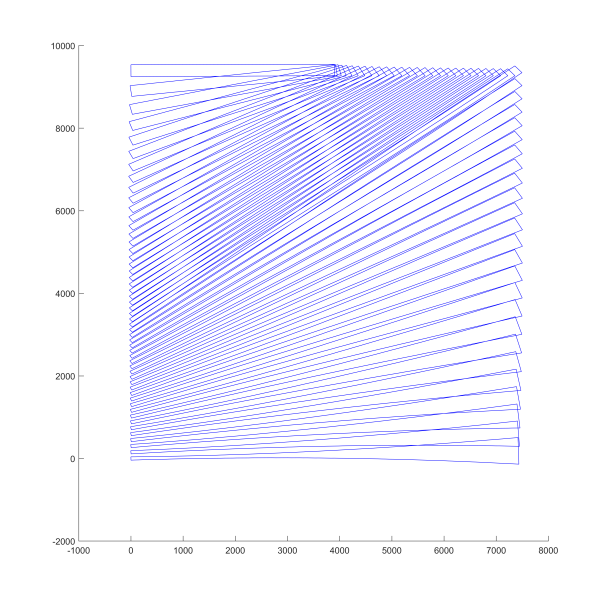
\includegraphics[width=0.4\linewidth]{media/image62}
		\caption{问题4的结果}
		\label{fig6}
	\end{figure}

在这样的测线设计下,测线总长度为392497.43米,侧漏海区占总待测海域面积的漏测率8.46\%,重叠率超过20\%部分的总长度为5642.33米。

\section{模型的评价与推广}
\subsection{模型的评价}
\subsubsection{模型的优点}
\begin{enumerate}
	\item 在进行各评价指标建模的过程中,建立了相对应的直角坐标系,这样的方法能够简化计算过程,并且更加具有依据性;
	\item 本文采用了动态多目标优化模型,该模型能在很短的时间内得到非常考破的结果,并且考虑到了多个目标之间的相互作用关系。
\end{enumerate}

\subsubsection{模型的缺点}
\begin{enumerate}
	\item 模型在某些计算过程中,进行了近似或者简化,这使得最终的结果与实际的结果之间存在偏差。
	\item 本文只对多波束测量模型进行理论上的分析,由于条件限制,并没有进行实际的测算与实验。不能完全保证模型的可靠性与准确性。
\end{enumerate}

\subsection{模型的推广}
本文主要采用了多目标动态规划模型,该模型能够考虑到系统中的多目标目标函数的影响,并且能够较短的时间内得到较为准确的结果,该模型可以推广到诸多其他领域的应用中,例如多目标水库调度优化、多目标TSP问题等。

\subsection{灵敏度分析}
在整个系统模型中,多波束换能器的开角始终是120°,但是在实际的操作或者实际的系统中,多波换能器的开角必定是可变的,对该参数进行灵敏度分析,分析不同的换能器开角下,问题四中测量长度的变化,具体的灵敏度分析结果如下表所示:
\begin{table}[H]
	\centering
	\caption{换能器开角的灵敏度分析}
	\label{tab3}
	\begin{tabular}{|c|c|c|c|c|}
		\hline
		换能器开角/° & 90        & 105      & 130      & 150      \\ \hline
		总测量长度/m & 1179859.3 & 599308.6 & 376792.9 & 227422.5 \\ \hline
	\end{tabular}
\end{table}

从上表可以看出,随着换能器开角的增加,总测量长度不段减小,且都在合理范围之内,认为该参数设置地比较合理,并且模型建立的比较稳定。这四组换能器开角的测线如下四图所示。
	\begin{figure}[H]
	\centering
	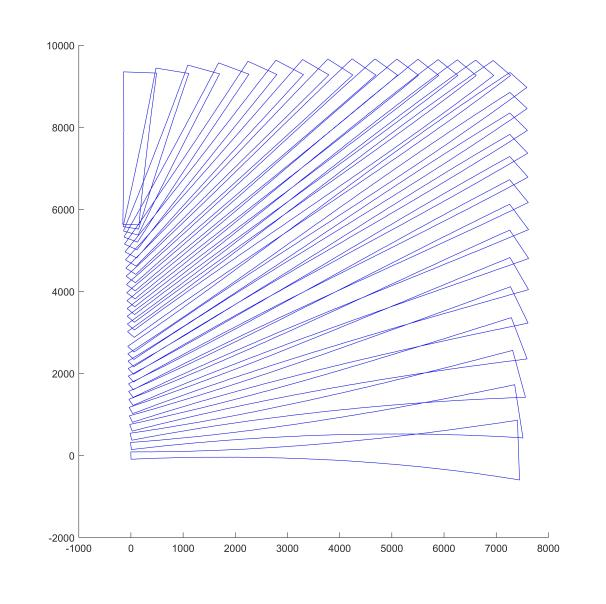
\includegraphics[width=0.35\linewidth]{media/image63}
	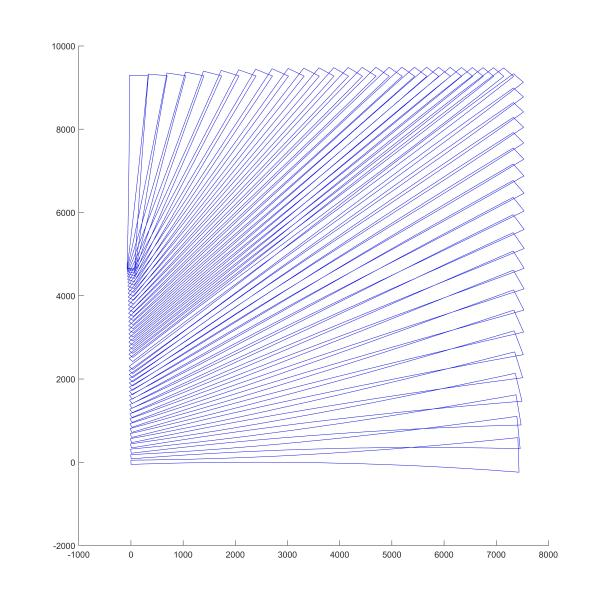
\includegraphics[width=0.35\linewidth]{media/image64}
	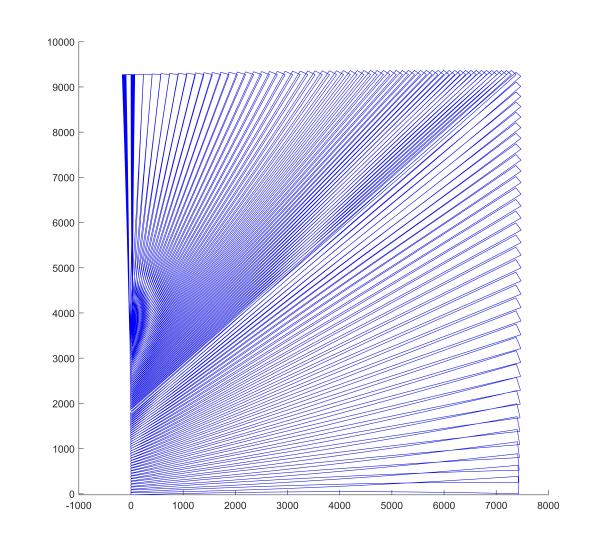
\includegraphics[width=0.35\linewidth]{media/image65}
	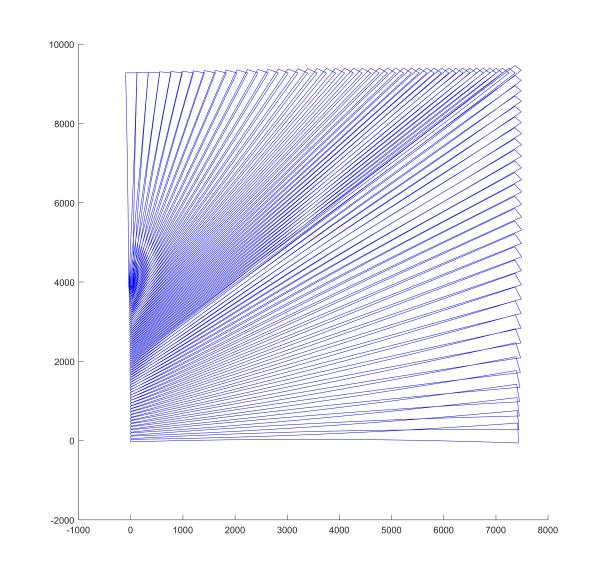
\includegraphics[width=0.35\linewidth]{media/image66}
	\caption{换能器开角分别为90°,105°,130°,150°时的测线}
	\label{fig7}
\end{figure}

\clearpage
\begin{thebibliography}{99}
	\bibitem{1}	王鑫. 水流引起的多波束测深误差改正方法研究[D].山东科技大学,2020.DOI:10.27275/d.cnki.gsdku.2020.000040.
\bibitem{2}	李欢. 组合导航船姿矫正在多波束测深中的应用研究[D].长安大学,2020.DOI:10.26976/d.cnki.gchau.2020.000984.
	\bibitem{3}	胡浩. 多波束测深自适应声速改正模型和方法研究[D].山东科技大学,2019.DOI:10.27275/d.cnki.gsdku.2019.000261.
	\bibitem{4}	周平. 多波束测深条带拼接区误差处理方法研究[D].东华理工大学,2017.
	\bibitem{5}	刘兆权.多波束测深精度评估[J].中国港湾建设,2017,37(05):63-67.
	\bibitem{6}	高君,肖付民,裴文斌等.多波束测深仪扫幅宽度评估方法[J].测绘科学技术学报,2013,30(01):28-32.
	\bibitem{7}	苏程. 深水多波束测深侧扫声纳显控系统研究[D].浙江大学,2012.
	\bibitem{8}	刘享明. 粒子滤波在多波束测深底跟踪中的应用研究[D].哈尔滨工程大学,2012.
	\bibitem{9}	朱小辰,刘雁春,肖付民等.多波束测深波束脚印位置归算模型研究[J].海洋测绘,2011,31(05):24-27.
	\bibitem{10}	朱小辰,刘雁春,肖付民等.多波束测深仪有效扇面宽度估计方法[J].海洋技术,2010,29(03):51-54.
\bibitem{11}	朱小辰,刘雁春,肖付民等.多波束测深全覆盖测量分辨率研究[J].测绘科学,2010,35(S1):22-24.DOI:10.16251/j.cnki.1009-2307.2010.s1.012.
\end{thebibliography}
\clearpage
\appendix
\section*{附录}
采用C编程,代码较多,此处仅演示部分。详见附录。
\begin{lstlisting}[caption={Q1.c},language=C]
#include "Q1.h"


void Q1(double eta_list[9])
{
	double DsCNS[9];
	int i;
	for (i = 0; i < 9; i++) {
		double d;
		eta_list[i] = 0.0;
		d = 70.0 - 0.026185921569186928 * (200.0 * (double)i + -800.0);
		DsCNS[i] = d;
		if (i + 1 != 1) {
			double eta_list_tmp;
			eta_list_tmp = DsCNS[i - 1];
			eta_list[i] = (-0.30470617011518009 * (eta_list_tmp / -0.960065624146096 +
			d / -0.94410760040152886) -
			(eta_list_tmp - d) / 0.026185921569186928) /
			(d * -0.30481062110221668 * -2.0831909295563458 *
			0.99965732497555726);
		}
	}
}
\end{lstlisting}
\begin{lstlisting}[caption={Q2.c},language=C]
#include "Q2.h"
#include <math.h>

void Q2(double saomiaodaikuan[64])
{
	static const double dv[8] = {0.0, 0.3, 0.6, 0.9, 1.2, 1.5, 1.8, 2.1};
	int i;
	int j;
	for (i = 0; i < 8; i++) {
		double DSW;
		double beta;
		beta = 45.0 * (double)i / 180.0 * 3.1415926535897931;
		DSW = tan(beta);
		DSW =
		atan(0.026185921569186928 * DSW / sqrt(DSW * DSW + 1.001371875164758));
		for (j = 0; j < 8; j++) {
			double Deepth;
			Deepth = dv[j] * 1852.0 * 0.026185921569186928 * cos(beta) + 120.0;
			saomiaodaikuan[i + (j << 3)] =
			0.8660254037844386 / sin(0.52359877559829893 - DSW) * Deepth +
			0.8660254037844386 / sin(DSW + 0.52359877559829893) * Deepth;
		}
	}
}
\end{lstlisting}
\begin{lstlisting}[caption={Q3.c},language=C]
/* Include Files */
#include "Q3.h"
#include "Q3_data.h"
#include "Q3_initialize.h"
#include "rand.h"

void Q3(void)
{
	int i;
	if (!isInitialized_Q3) {
		Q3_initialize();
	}
	for (i = 0; i < 18; i++) {
		b_rand();
		b_rand();
	}
	for (i = 0; i < 18; i++) {
		b_rand();
		b_rand();
	}
}	
\end{lstlisting}

\end{document}